\documentclass{beamer}
\usepackage[utf8]{inputenc}
\usepackage[T1]{fontenc}
\usepackage{graphicx}
\usepackage{tcolorbox}
\usepackage{hyperref}
\hypersetup{
    colorlinks=true,
    linkcolor=pink,
    urlcolor=cyan,
    urlbordercolor=cyan,
}
\graphicspath{ {./images/} }

\usetheme{Arguelles}

\title{Tutorial 2}
\subtitle{CS3241 Computer Graphics (AY23/24)}
\date{\today}
\author{Wong Pei Xian}
\institute[]{\email{e0389023@u.nus.edu}}

\begin{document}

\frame[plain]{\titlepage}

\begin{frame}[plain,standout]
    \AlegreyaExtraBold \LARGE
    Attendance taking
\end{frame}

\section{Question 1}

\begin{frame}
    \frametitle{Question 1}
    What is a GLUT \textbf{display callback} function?  
    Give example \textbf{events} for which the display callback function should be called.
\end{frame}

\begin{frame}
    \frametitle{GLUT function}

    \begin{tcolorbox}
        \textbf{GLUT}: OpenGL Utility Toolkit (Lecture 2 slide 10), \\
        
        a library that provides \textbf{I/O functionality} common to \textcolor{teal}{all window systems}.
    \end{tcolorbox}

    \begin{center}
        
\includegraphics[]{q1-glut-callbacks.png}
    \end{center}

\end{frame}

\begin{frame}
    \frametitle{GLUT display callback}

    \begin{tcolorbox}
        \centering
        \texttt{glutDisplayFunc(void (*func)(void))}.
    \end{tcolorbox}

    \begin{itemize}
        \item Takes in a function pointer to user defined display method \texttt{func}.
        \item Executed on each window refresh.
        \item \href{https://www.opengl.org/resources/libraries/glut/spec3/node46.html}{OpenGL reference}
    \end{itemize}

\end{frame}

\section{Question 2}

\begin{frame}
    \frametitle{Question 2}

    What is the use of the GLUT function \texttt{glutPostRedisplay()}?

\end{frame}

\begin{frame}
    \frametitle{\texttt{glutPostRedisplay}}

    \begin{tcolorbox}
        \textit{Redisplay}: Update of the display output (usually due to a change in internal state).
    \end{tcolorbox}

    The execution of the \texttt{glutPostRedisplay()} function tells GLUT to call the 
    display callback function at the end of the current event loop. \\

    \begin{itemize}
        \item Sets the redisplay state.
        \item Multiple calls to \texttt{glutPostRedisplay} simply set the redisplay state multiple times (coalesce multiple display function calls)
        \item the display callback is only called once on the next cycle.
    \end{itemize}

\end{frame}

\begin{frame}
    \frametitle{\texttt{glutPostRedisplay}}

    \begin{center}
        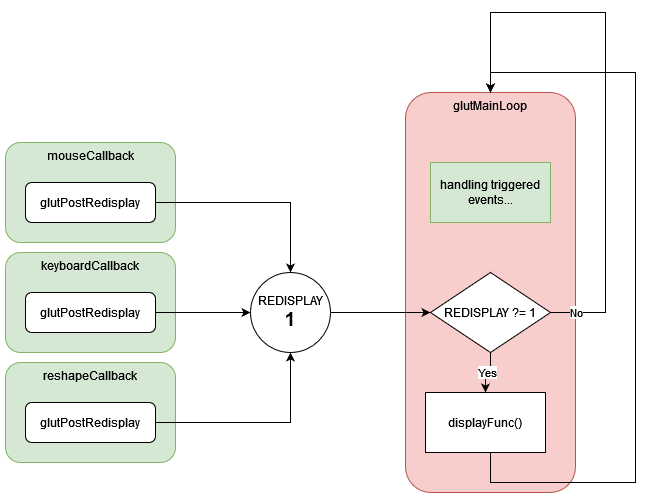
\includegraphics[scale=0.3]{images/glutPostRedisplay.png}
    \end{center}

\end{frame}

\section{Question 3}

\begin{frame}
    \frametitle{Question 3}
    How does double buffering work?
\end{frame}

\begin{frame}
    \frametitle{Double buffering}

    \begin{center}
        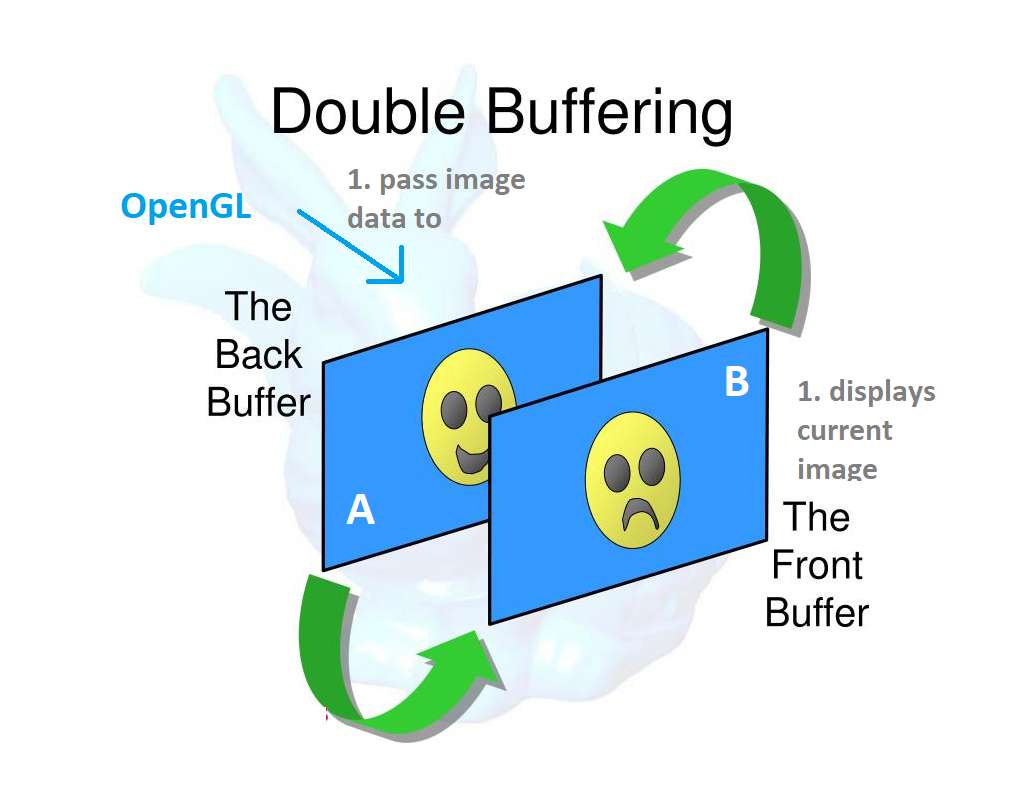
\includegraphics[scale=0.4]{q3-step1.png}
    \end{center}

    \begin{itemize}
        \item \textcolor{red}{Back} buffer: \textcolor{red}{apply} graphics \textbf{WHILE}
        \item \textcolor{blue}{Front} buffer: \textcolor{blue}{display} graphics 
    \end{itemize}

\end{frame}

\begin{frame}
    \frametitle{Double buffering}

    \begin{center}
        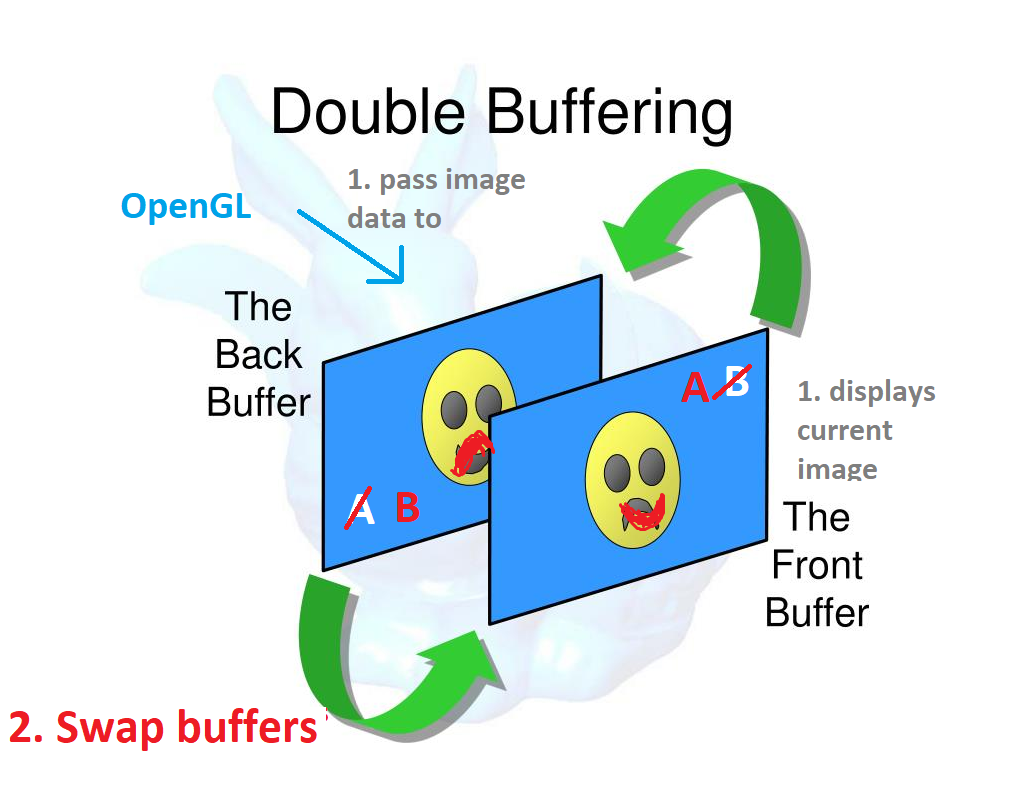
\includegraphics[scale=0.4]{q3-step2.png}
    \end{center}

    \textbf{No "incomplete" frames will be visible,} 
    as the swap is only performed after the the back buffer is filled.

\end{frame}

\begin{frame}
    \frametitle{Question 3}

    Why do we use double buffering?

\end{frame}

\begin{frame}
    \frametitle{Prevents screen tearing}

    \begin{center}
        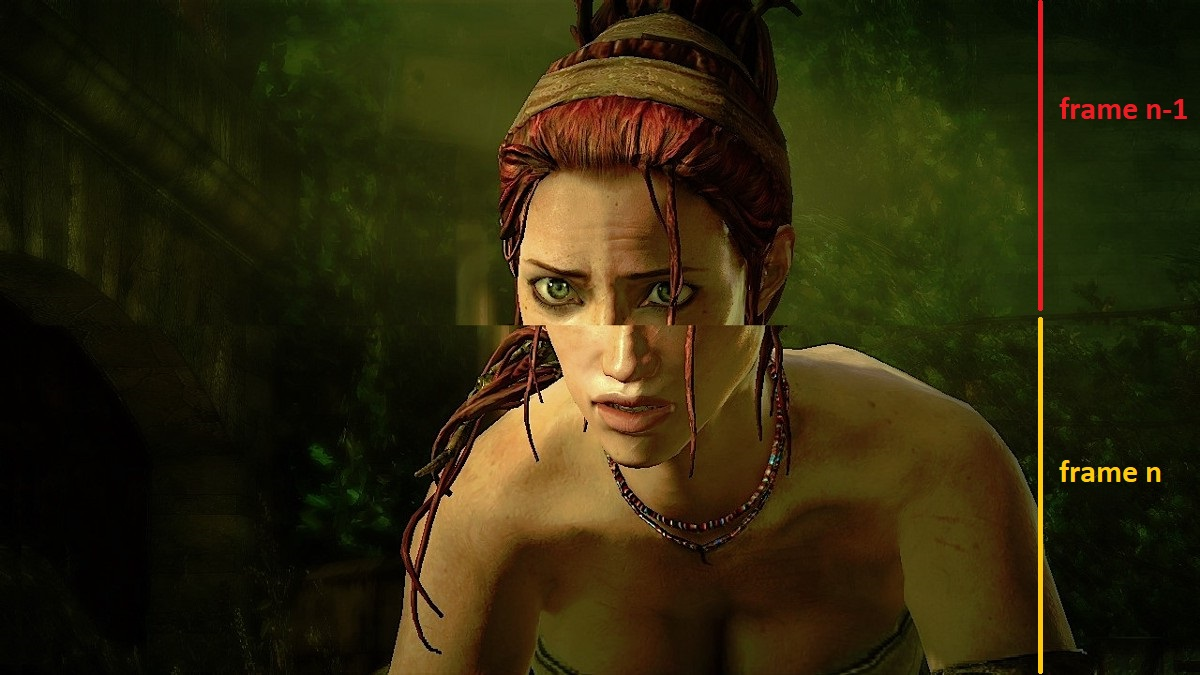
\includegraphics[scale=0.3]{screen-tear.jpg}
    \end{center}

    \begin{tcolorbox}
        \textbf{Screen tearing}: 
        when the rate of graphics feed application $\neq$ window refresh rate.
    \end{tcolorbox}

\end{frame}

\begin{frame}
    \frametitle{Double buffering in OpenGL}

    To enable double buffering: \texttt{glutInitDisplayMode}.\\

    To perform the buffer swap in display function: \texttt{glutSwapBuffers}.\\

    \textit{See lecture 3 slide 14.}

\end{frame}

\section{Question 4}

\begin{frame}
    \frametitle{Question 4}
    The use of any special hidden surface removal method is not necessary if we can sort the polygons in a back-to-front order 
    and render these polygons in that order. (Tutorial 1 Q6)\\

    \vspace{1em}
    
    Is it \textbf{always possible} that any set of polygons can be sorted in a back-to-front order?
\end{frame}

\begin{frame}
    \frametitle{Cyclic overlap}

    \begin{center}
        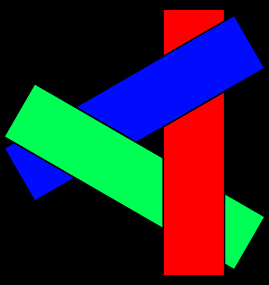
\includegraphics[scale=0.6]{cyclic-overlap.png}
    \end{center}

\end{frame}

\section{Question 5}

\begin{frame}
    \frametitle{Question 5a}

    (A) What is an OpenGL viewport?
\end{frame}

\begin{frame}
    \frametitle{Viewport}

    \begin{tcolorbox}
        OpenGL viewport: A rectangular region of the window in which OpenGL can draw.
    \end{tcolorbox}

\end{frame}

\begin{frame}
    \frametitle{Question 5b}

    (B) How do you specify one?
\end{frame}

\begin{frame}
    \frametitle{\texttt{glViewport}}

    \begin{center}
        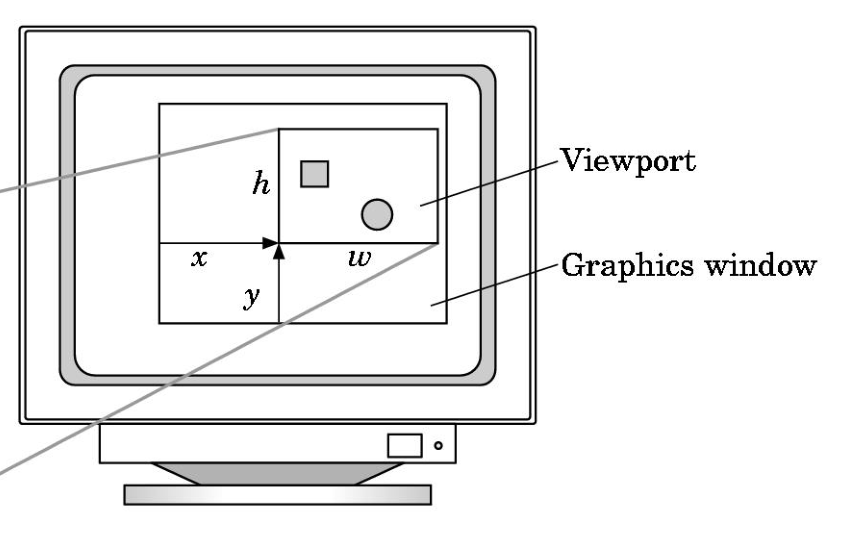
\includegraphics[scale=0.3]{viewport.png}
    \end{center}

    \begin{tcolorbox}
        \begin{center}
            \texttt{glViewport(GLint x, GLint y, GLsizei w, GLsizei h)}
        \end{center}
    \end{tcolorbox}

    Note: $x,y,w,h$ are in window coordintes.

\end{frame}

\begin{frame}
    \frametitle{Question 5c}

    (C) Can we have \textbf{multiple viewports} in one window?
\end{frame}

\begin{frame}
    \frametitle{Yes!}

    \begin{center}
        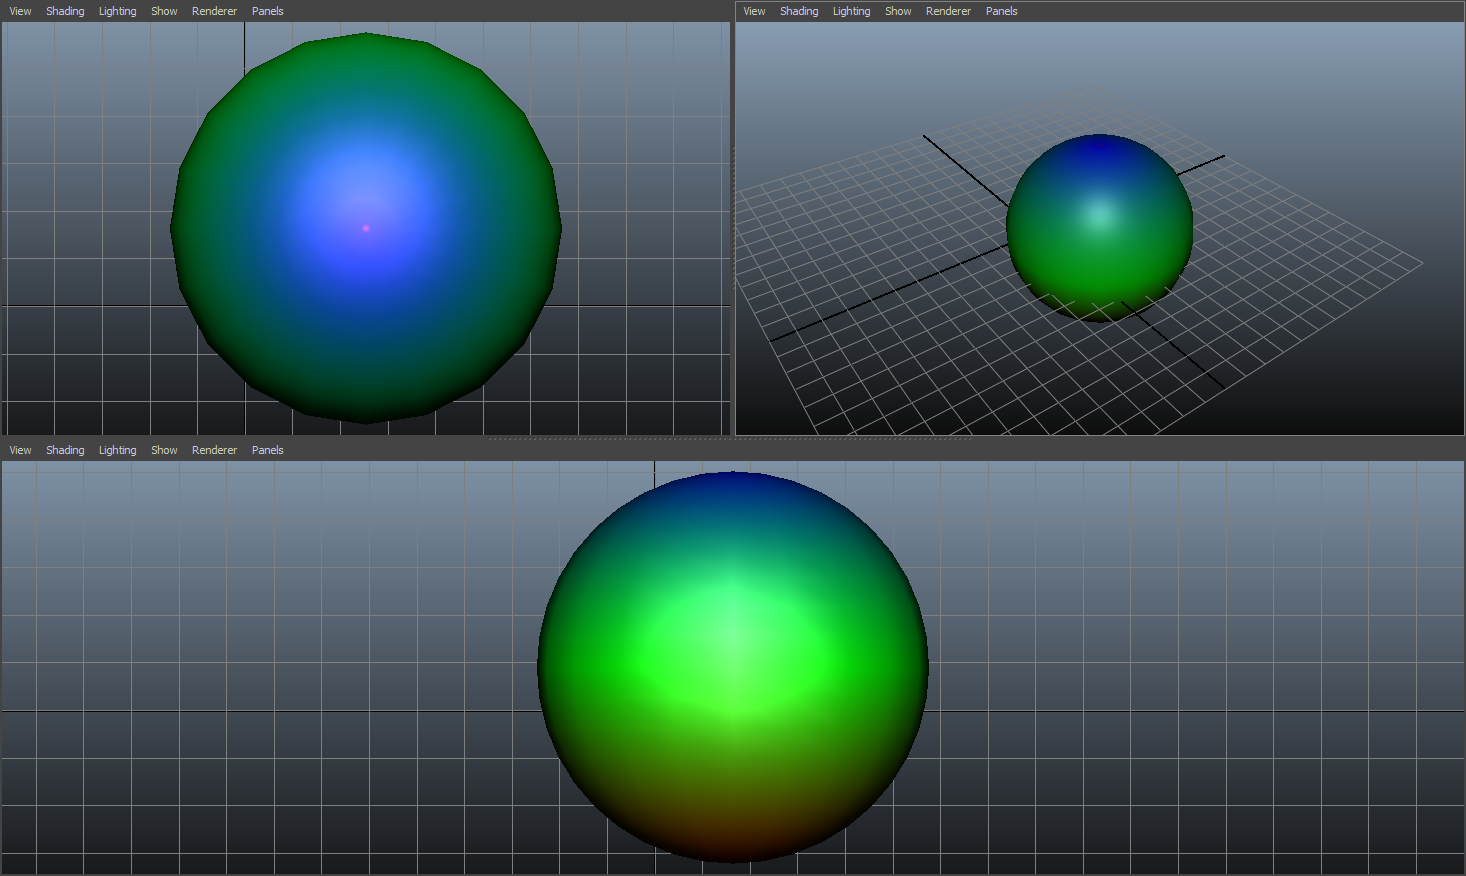
\includegraphics[scale=0.3]{multiple-viewports.png}
    \end{center}

    [3DSMax] Each viewport has a different perspective of the same world.

\end{frame}

\begin{frame}
    \frametitle{Yes!}

    \begin{center}
        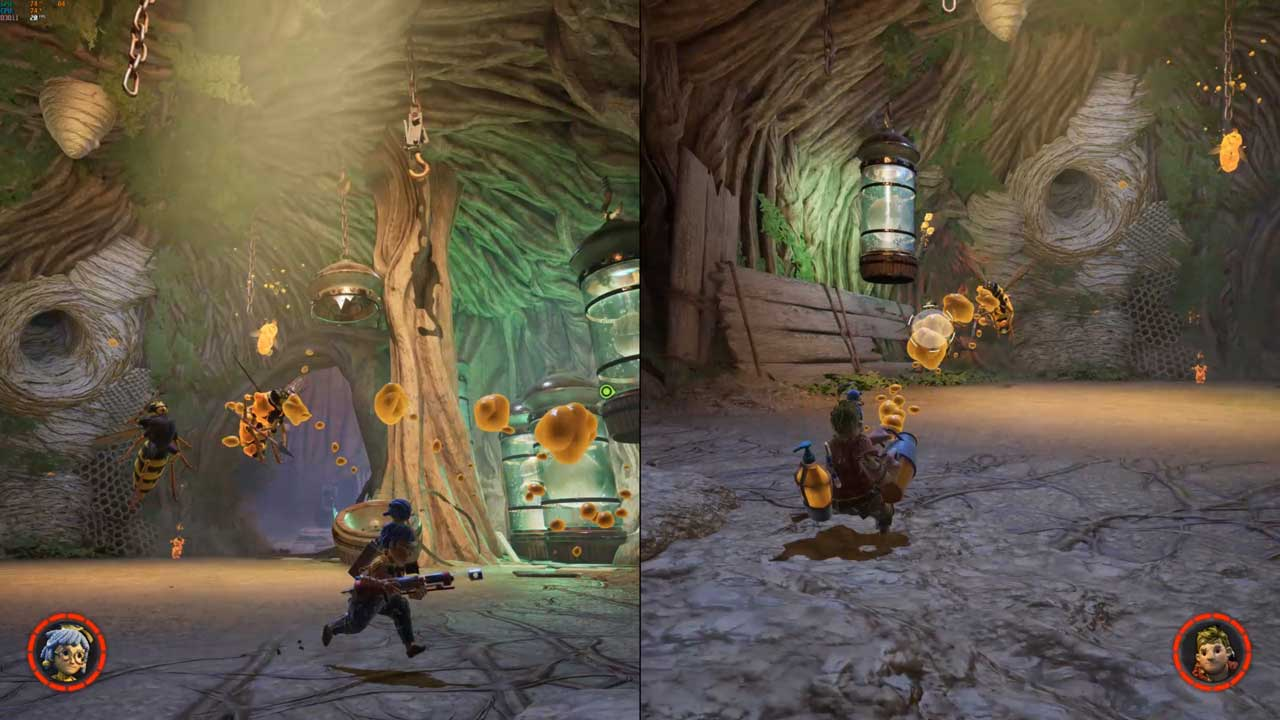
\includegraphics[scale=0.2]{it-takes-two.jpg}
    \end{center}

    [It Takes Two] Different camera movements possible.

\end{frame}

\begin{frame}
    \frametitle{Question 5d, 5e}

    (D) Can a viewport be larger than the window? \\

    \vspace{1em}

    (E) If yes, what will happen?
\end{frame}

\begin{frame}
    \frametitle{Yes!}

    \begin{center}
        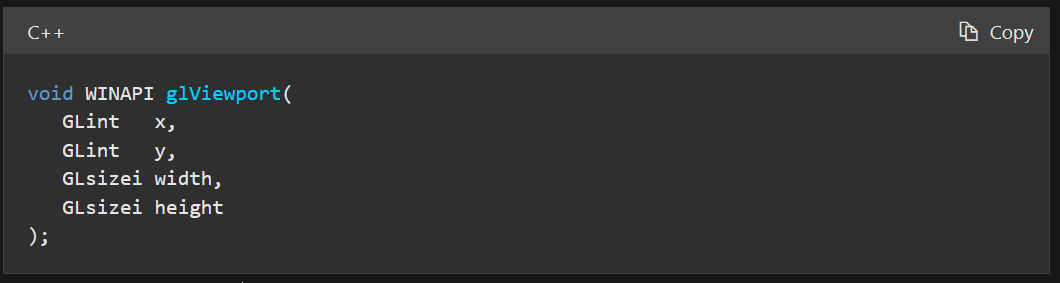
\includegraphics[scale=0.5]{glviewport.png}
    \end{center}

    Parameter types are \texttt{GLint} for x and y coordinates, so they can be negative and go out of the screen.\\

    \vspace{1em}

    Or \texttt{width} or \texttt{height} could also exceed window size.

    \textbf{Viewport size is independent of window size.}

\end{frame}

\begin{frame}
    \frametitle{Specification example}

    \begin{center}
        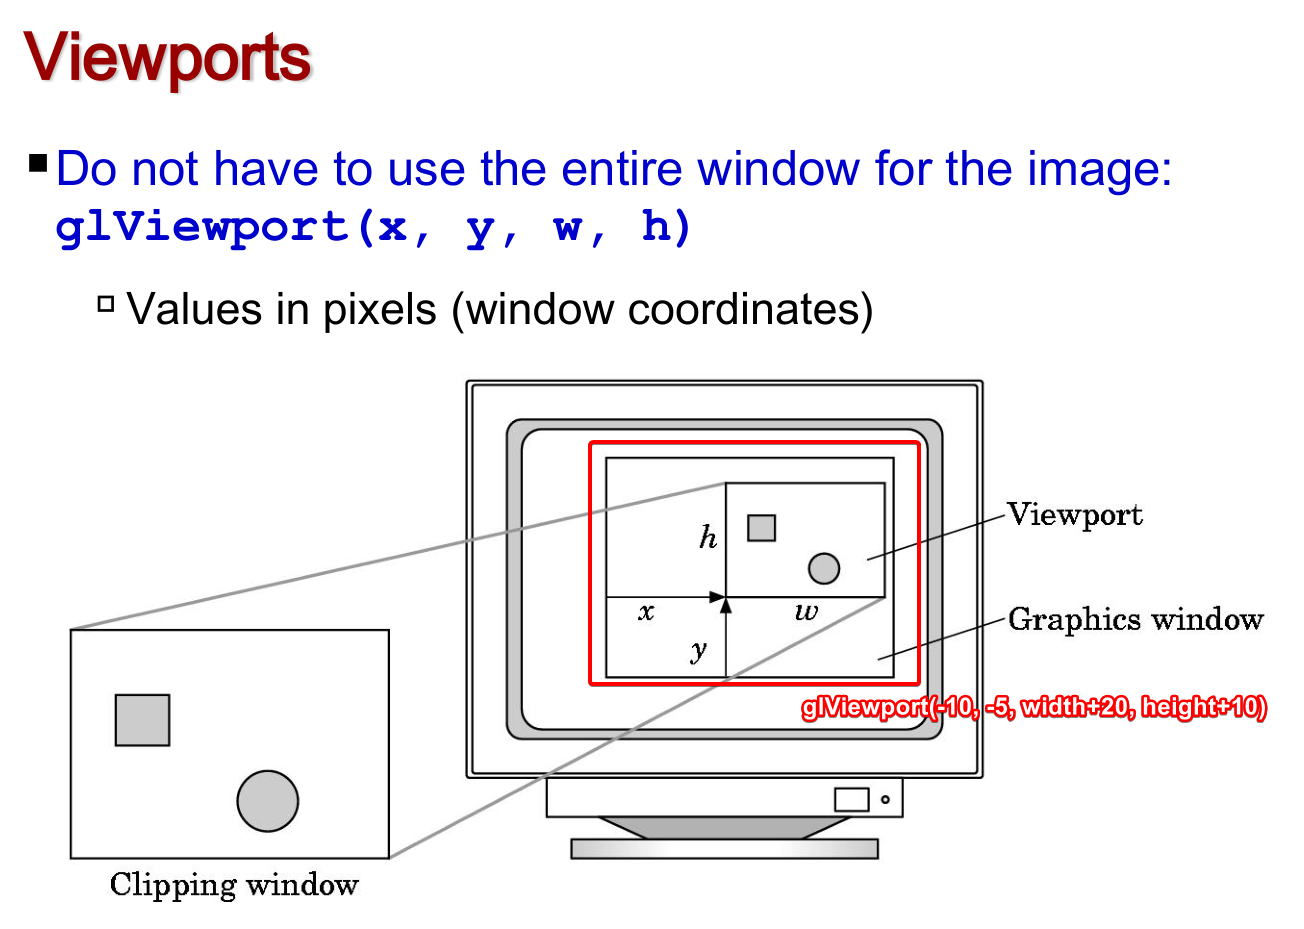
\includegraphics[scale=0.3]{viewport-window.png}
    \end{center}

    Consequence is that the viewport will be clipped by the window.
    
\end{frame}

\begin{frame}
    \frametitle{Question 5f}

    (F) When you use \texttt{glClear(GL\_COLOR\_BUFFER\_BIT)},
    are you clearing the entire window or just the viewport?
\end{frame}

\begin{frame}
    \frametitle{Question 5f}

    When you use \texttt{glClear(GL\_COLOR\_BUFFER\_BIT)},
    are you clearing the entire window or just the viewport?

    \begin{tcolorbox}
        Short answer: the window.

        Long answer: \texttt{glClear(mask)} marks the \textbf{buffer} to be cleared.
        The buffer is associated with the \textbf{window} i.e. the (physically) visible area, 
        not the (virtual) viewport.
    \end{tcolorbox}
\end{frame}

\section{Question 6}

\begin{frame}
    \frametitle{Question 6}

    Assume we have the following OpenGL function calls:

    \begin{tcolorbox}
        \texttt{\\
            glViewport( u, v, w, h ); \\
            ... \\
            gluOrtho2D( x\_min, x\_max, y\_min, y\_max );\\
        }
    \end{tcolorbox}

    Find the mathematical expressions that map a point $(x, y)$ that lies within the 
    clipping rectangle to a point $(xs, ys)$ that lies within the viewport.
\end{frame}

\begin{frame}
    \frametitle{Clip space to window space}

    \begin{center}
        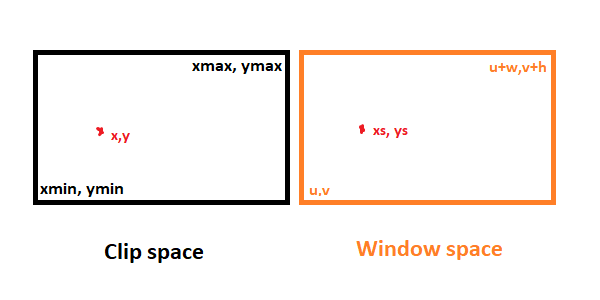
\includegraphics[]{clip-window.png}
    \end{center}
    
    $x_s = u + (x-x_{\min}) (\frac{w}{x_{\max} - x_{\min}})$\\
    $y_s = v + (y-y_{\min}) (\frac{h}{y_{\max} - y_{\min}})$\\

\end{frame}

\section{Question 7}

\begin{frame}
    \frametitle{Question 7a}
    In many old CRT monitors, the pixels are not square. 
    Let’s assume the pixel width-to-height aspect ratio is 4:3. 
    \vspace{1em}

    Suppose in the \textbf{camera coordinate frame}, there is a disc in the z = 0 plane, 
    centered at (100, 200, 0), and has a radius of 10. 

    You want to draw the entire disc as big as possible inside the window, 
    and it should appear circular and not oval.
    \vspace{1em}

    \begin{tcolorbox}
        If the window size is \underline{\quad\quad}, how would you set up the \textcolor{teal}{viewport} and the
        \textcolor{violet}{orthographic projection} using OpenGL?
        \begin{itemize}
            \item 600 $\times$ 300
            \item 300 $\times$ 600
            \item 300 $\times$ 320
        \end{itemize}
    \end{tcolorbox}
\end{frame}

\begin{frame}
    \frametitle{Template}

    \begin{center}
        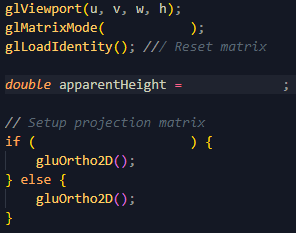
\includegraphics[scale=1.4]{q7.png}
    \end{center}

\end{frame}

\begin{frame}
    \frametitle{Visualize}

    \begin{center}
        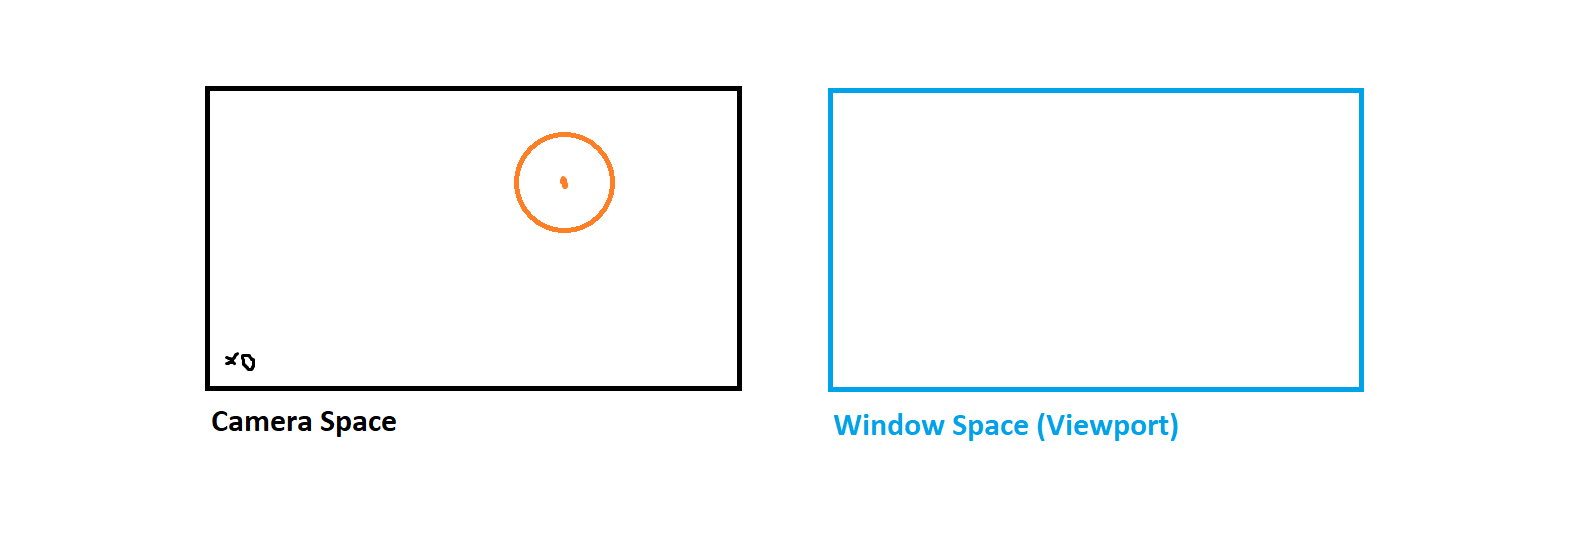
\includegraphics[scale=0.4]{q7-cam-win.png}
    \end{center}

    \begin{tcolorbox}
        Consider the case where the pixels are square first.
        Let $w, h$ be the width and height of the viewport, 
        $c$ be the 2D coordinates of the center of the circle,
        and $r$ be the radius.
    \end{tcolorbox}

\end{frame}

\begin{frame}
    \frametitle{}

    \begin{center}
        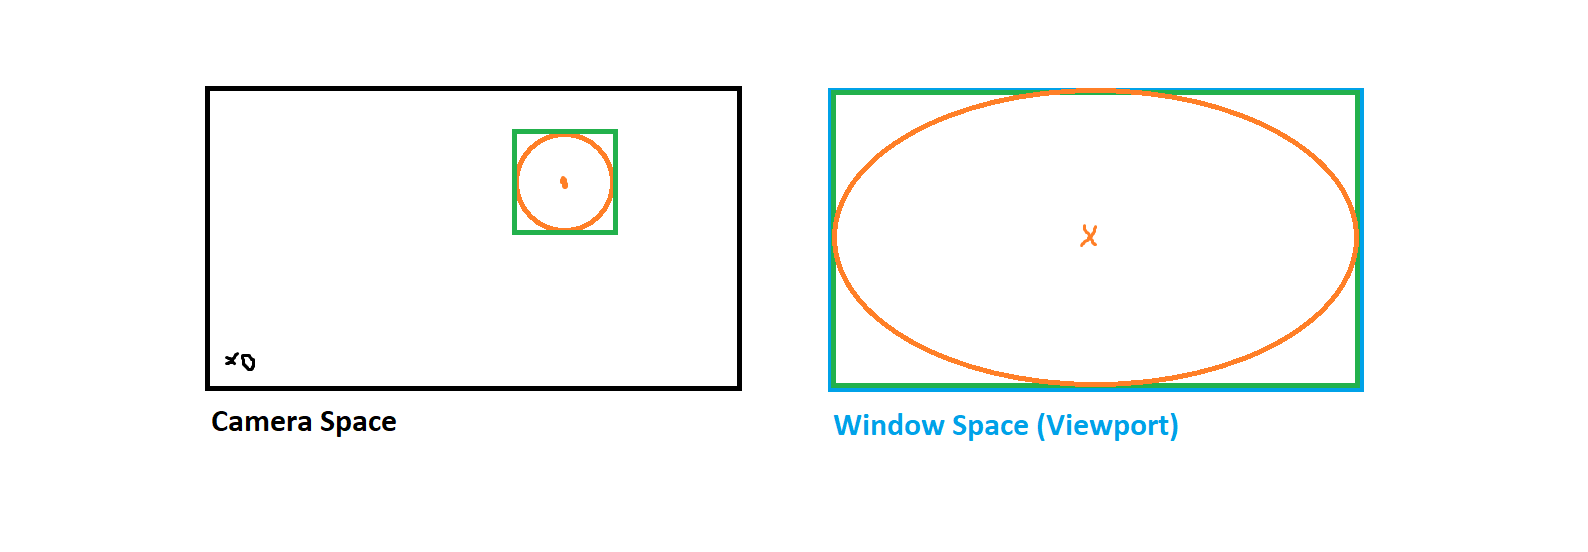
\includegraphics[scale=0.4]{q7-cam-win-1.png}
    \end{center}

    \begin{tcolorbox}
        \small
        \texttt{glViewport(0, 0, w, h);}\\
        \texttt{glOrtho(c.x - r, c.x + r, c.y - r, c.y + r);}
    \end{tcolorbox}

\end{frame}

\begin{frame}
    \frametitle{}

    \begin{center}
        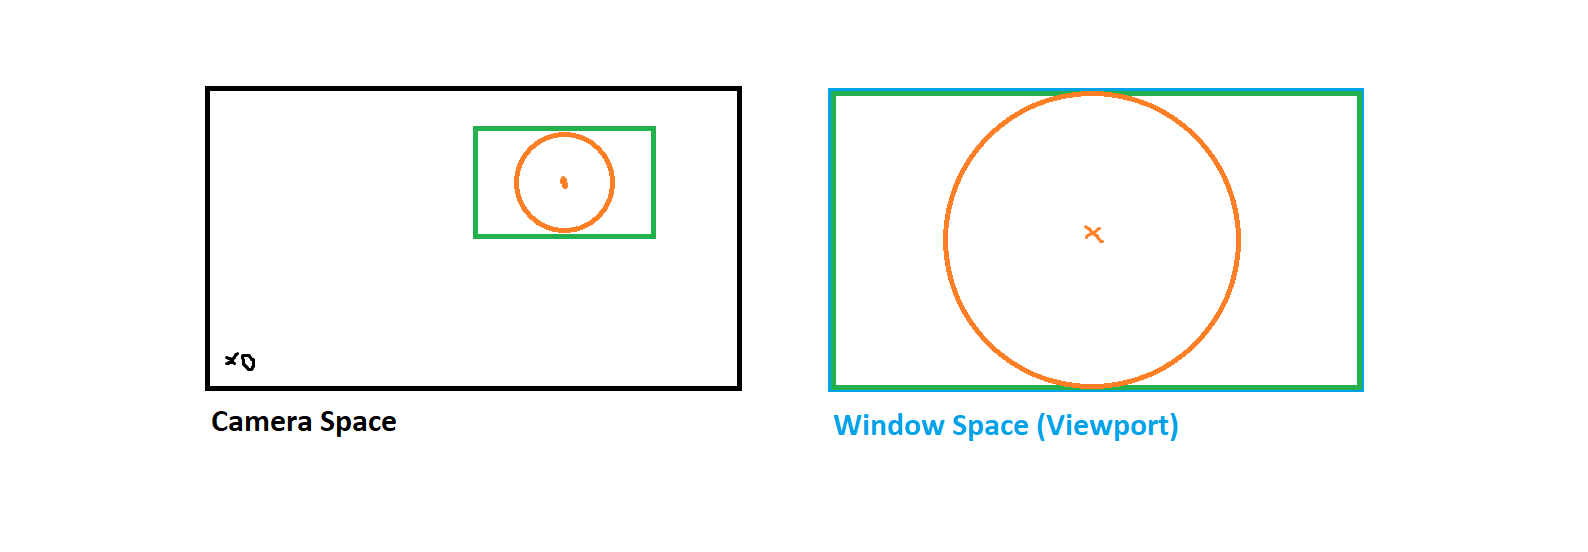
\includegraphics[scale=0.4]{q7-cam-win-2.png}
    \end{center}

    \begin{tcolorbox}
        \small
        Assuming the pixels are square, to get this we can:\\
        \texttt{glViewport(0, 0, w, h);}\\
        \texttt{glOrtho(c.x - r \textcolor{teal}{* w/h} , c.x + r \textcolor{teal}{* w/h}, \\
            c.y - r, c.y + r);}
    \end{tcolorbox}

\end{frame}

\begin{frame}
    \frametitle{}

    \begin{center}
        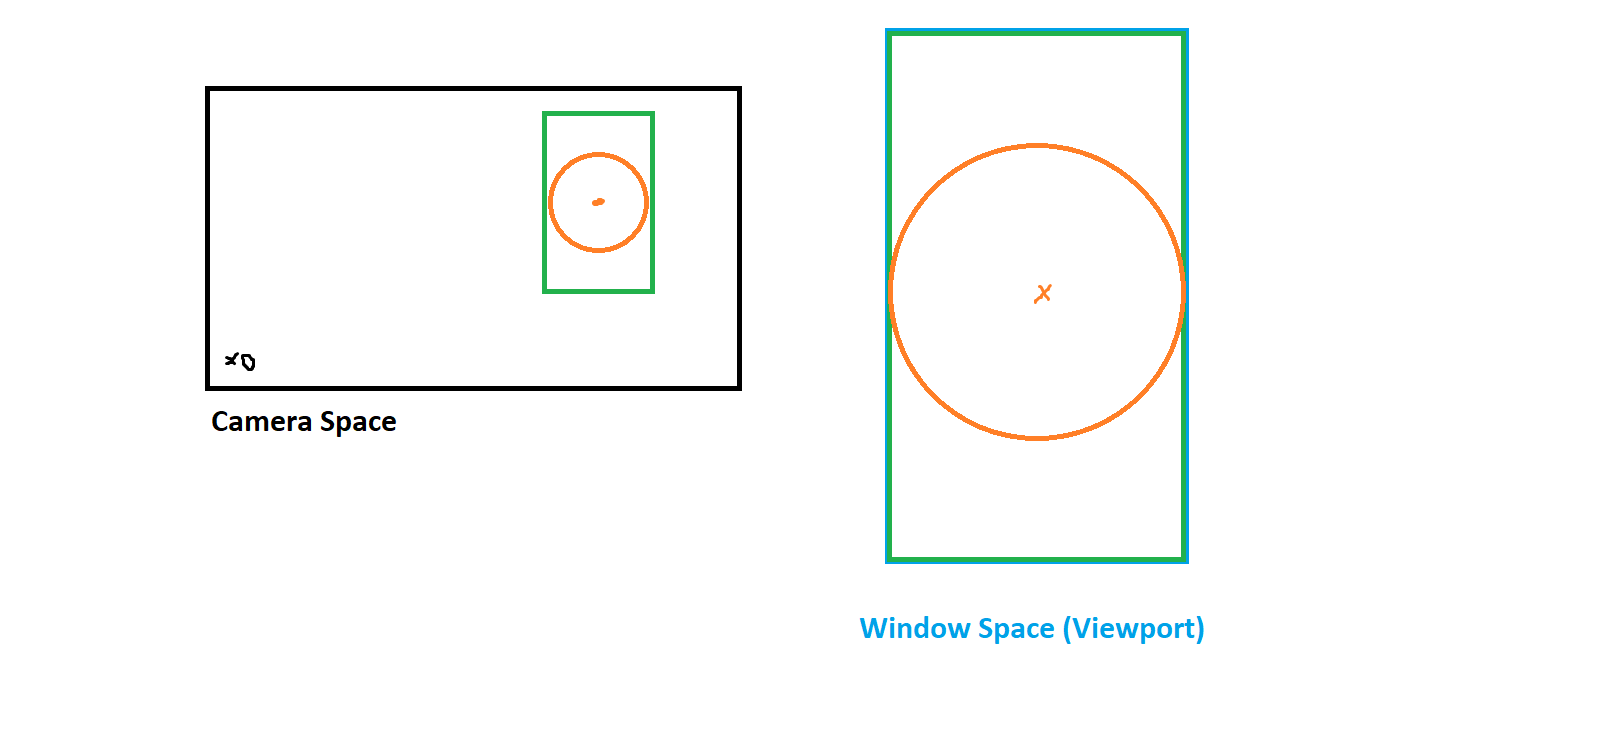
\includegraphics[scale=0.4]{q7-cam-win-3.png}
    \end{center}

    \begin{tcolorbox}
        \small
        Assuming the pixels are square, to get this we can:\\
        \texttt{glViewport(0, 0, w, h);}\\
        \texttt{glOrtho(c.x - r , c.x + r, \\
        c.y - r \textcolor{teal}{* h/w}, c.y + r \textcolor{teal}{* h/w});}
    \end{tcolorbox}

\end{frame}

\begin{frame}
    \frametitle{What if we consider the 4:3 pixels?}

    Then we have to make sure the clipping space scales to the 
    \textbf{apparent aspect ratio}, i.e. $\texttt{apparentWidth} = w \times \frac{4}{3}$.

\end{frame}

\begin{frame}
    \frametitle{}

    \begin{center}
        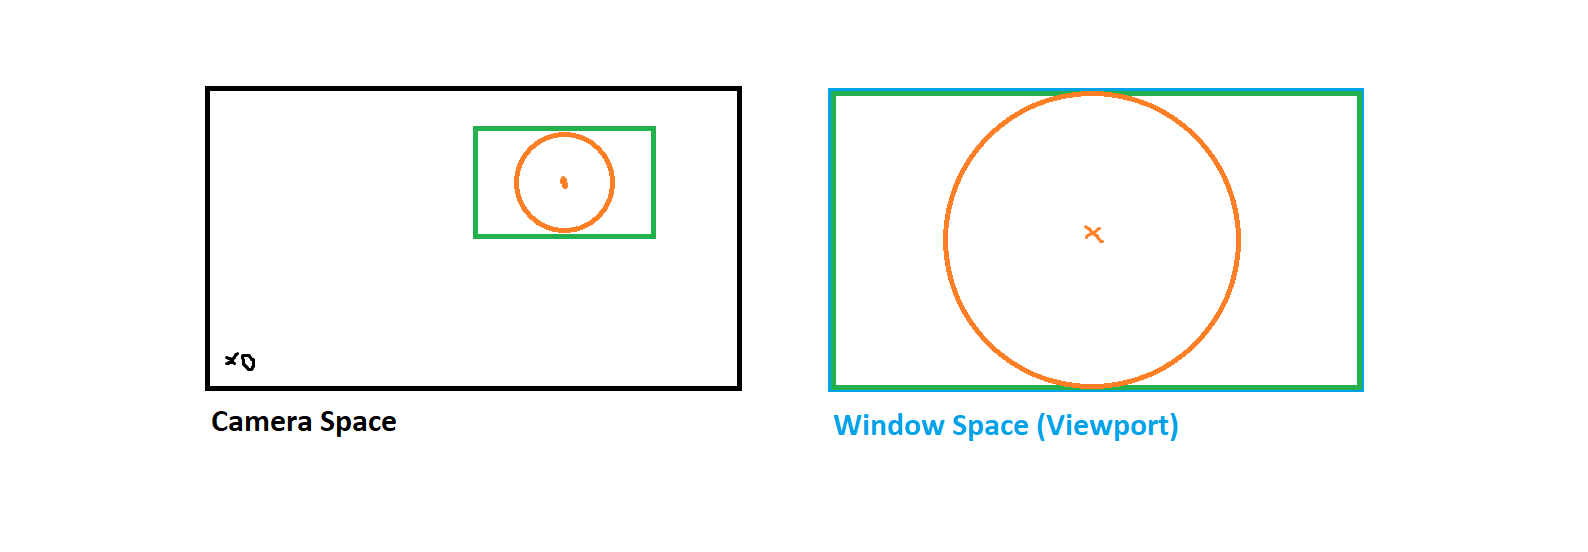
\includegraphics[scale=0.4]{q7-cam-win-2.png}
    \end{center}

    \begin{tcolorbox}
        \small
        Assuming the pixels are \textcolor{red}{4:3}, to get this we can:\\
        \texttt{glViewport(0, 0, w, h);}\\
        \texttt{glOrtho(c.x - r \textcolor{red}{* \texttt{apparentWidth}/h} , \\
        c.x + r \textcolor{red}{* \texttt{apparentWidth}/h}, c.y - r, c.y + r);}
    \end{tcolorbox}

\end{frame}

\begin{frame}
    \frametitle{}

    \begin{center}
        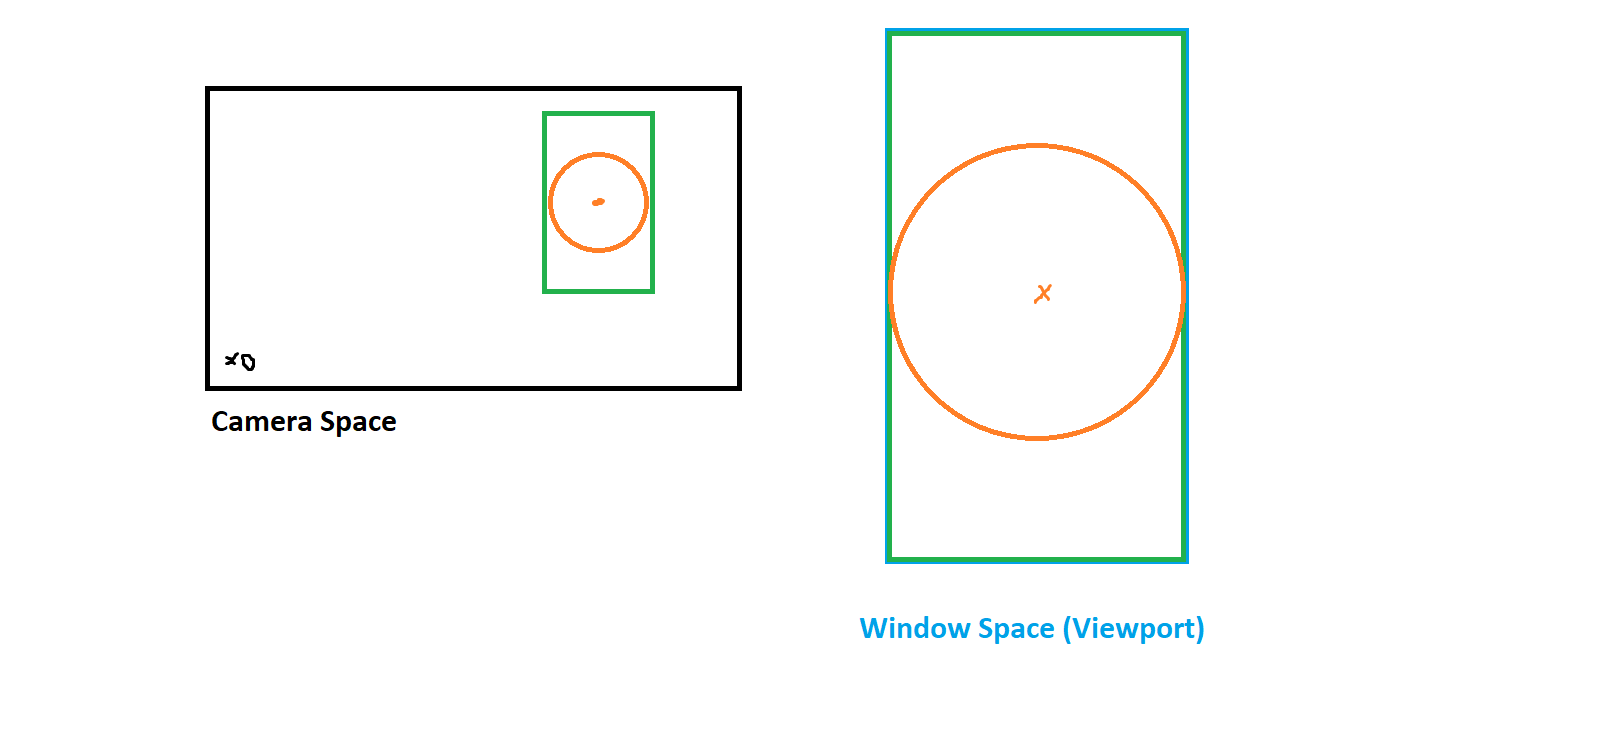
\includegraphics[scale=0.4]{q7-cam-win-3.png}
    \end{center}

    \begin{tcolorbox}
        \small
        Assuming the pixels are \textcolor{red}{4:3}, to get this we can:\\
        \texttt{glViewport(0, 0, w, h);}\\
        \texttt{glOrtho(c.x - r , c.x + r, \\
        c.y - r \textcolor{red}{* h/\textcolor{red}{apparentWidth}},\\
        c.y + r \textcolor{red}{* h/\textcolor{red}{apparentWidth}});}
    \end{tcolorbox}

\end{frame}

\begin{frame}
    \frametitle{Key takeaway}

    In 2D orthographic projecton, \textcolor{teal}{aspect ratios must match} between 
    the clipping space and the window space (\textbf{assuming uniform pixels})
    to not be distorted.

    \begin{tcolorbox}
        If the window size is \underline{\quad\quad}, how would you set up the \textcolor{teal}{viewport} and the
        \textcolor{violet}{orthographic projection} using OpenGL?
        \begin{itemize}
            \item 600 $\times$ 300 $\rightarrow \textbf{800} \times 300$ \textbf{(horizontal)}
            \item 300 $\times$ 600 $\rightarrow \textbf{400} \times 600$ \textbf{(vertical)}
            \item 300 $\times$ 320 $\rightarrow \textbf{400} \times 320$ \textbf{(horizontal)}
        \end{itemize}
    \end{tcolorbox}

\end{frame}

\begin{frame}
    \frametitle{Alternative: scaled viewport}

    \begin{center}
        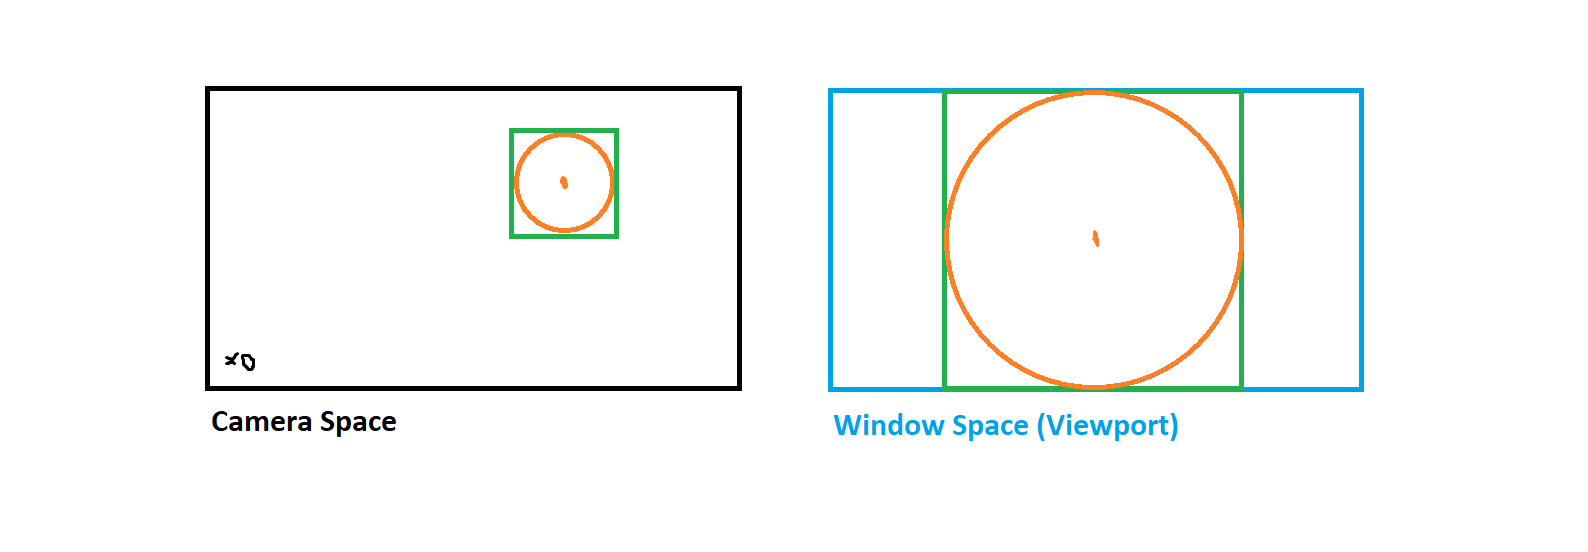
\includegraphics[scale=0.3]{q7-cam-win-4.png}
    \end{center}

    \begin{tcolorbox}
        \small
        The pixels are \textcolor{red}{4:3}.\\
        \texttt{int squishedWidth = w * 3/4;}\\
        \texttt{glViewport(0, \textcolor{red}{w / 2 - squishedWidth / 2}, \textcolor{red}{squishedWidth}, h);}\\
        \texttt{glOrtho(c.x - r , c.x + r, c.y - r, c.y + r);}
    \end{tcolorbox}

    You can similarly account for the case where $h > w$.

\end{frame}

\ThankYou
\begin{frame}[plain,standout]
    Thanks! Get the slides here after the tutorial.\\
    \vspace{2em}
    \scalebox{3}{\faGithub}\par\bigskip
    \url{https://trxe.github.io/cs3241-notes}
\end{frame}

\end{document}